\header{
    \section{Bois de l'arbois} \label{bois-de-l-arbois}
    %
    \insertComment{Chanson de Pierre Dastro-Geze (1925-1984).}{L'arbois est un vin AOC du Jura.}
}

\enluminure{4}{\href{https://www.youtube.com/watch?v=Zb7e8wGw1og}{S}}{ur mon} coteau, y a de la vigne
\\Dans mon tonneau, y a le bon vin (le bon vin)
\\Plus j'en bois, plus j'ai bonne mine
\\Plus j'en bois, plus je me sens bien
\\C'est le bon vin de mon pays
\\C'est lui le soleil de ma vie
\\C'est mon ami et dans mon cœur
\\C'est lui qui fait tout mon bonheur
\\Quand ma Lison me répond non
\\C'est encore lui qui me dit oui
\\Sautez bouchons, videz flacons
\\Chantons, chantons à ma chanson
\\\\\textbf{Refrain :}
\\Dans tous les cas mon gars
\\Bois de l'Arbois, tu l'auras belle
\\Dans tous les cas, mon gars
\\Plus on en boit, plus on va droit
\\
\bisdouble{Bois, bois, la vie sera belle}
{Bois, bois, bois du vin d'Arbois}
\\Du vin d'Arbois !
\breakpage
\\\\Sur mon coteau, y a ma Lisette
\\Sa peau est douce et son teint frais (son teint frais)
\\Elle est si belle et gentillette
\\Que jamais je ne l'oublierai
\\C'est mon béguin, c'est mon amour
\\Le seul objet de mes désirs
\\Son cœur m'a séduit pour toujours
\\Je lui ferai tout son plaisir
\\Cloches, sonnez, carillonnez
\\Car nous allons nous marier
\\J'aime le vin, mais nom de nom
\\J'aime encore mieux ma Lison
\\\\Sur mon coteau y a un pauvre homme
\\Abandonné par sa Lison (sa Lison)
\\Elle l'a trompé, la friponne
\\Avec son ami vigneron
\\Fini l'amour, plus de jupon
\\Je vais retrouver la raison
\\Et ma raison, c'est le bon vin
\\C'est la vigne et son jus divin
\\Holà, patron et qu'on me verse
\\Un coup de ce raisin béni
\\Ma vigne est là, c'est ma maîtresse
\\Et le bon vin, c'est mon ami
\\\\\textbf{Refrain x2}
\vspace{0.5cm}
\begin{center}
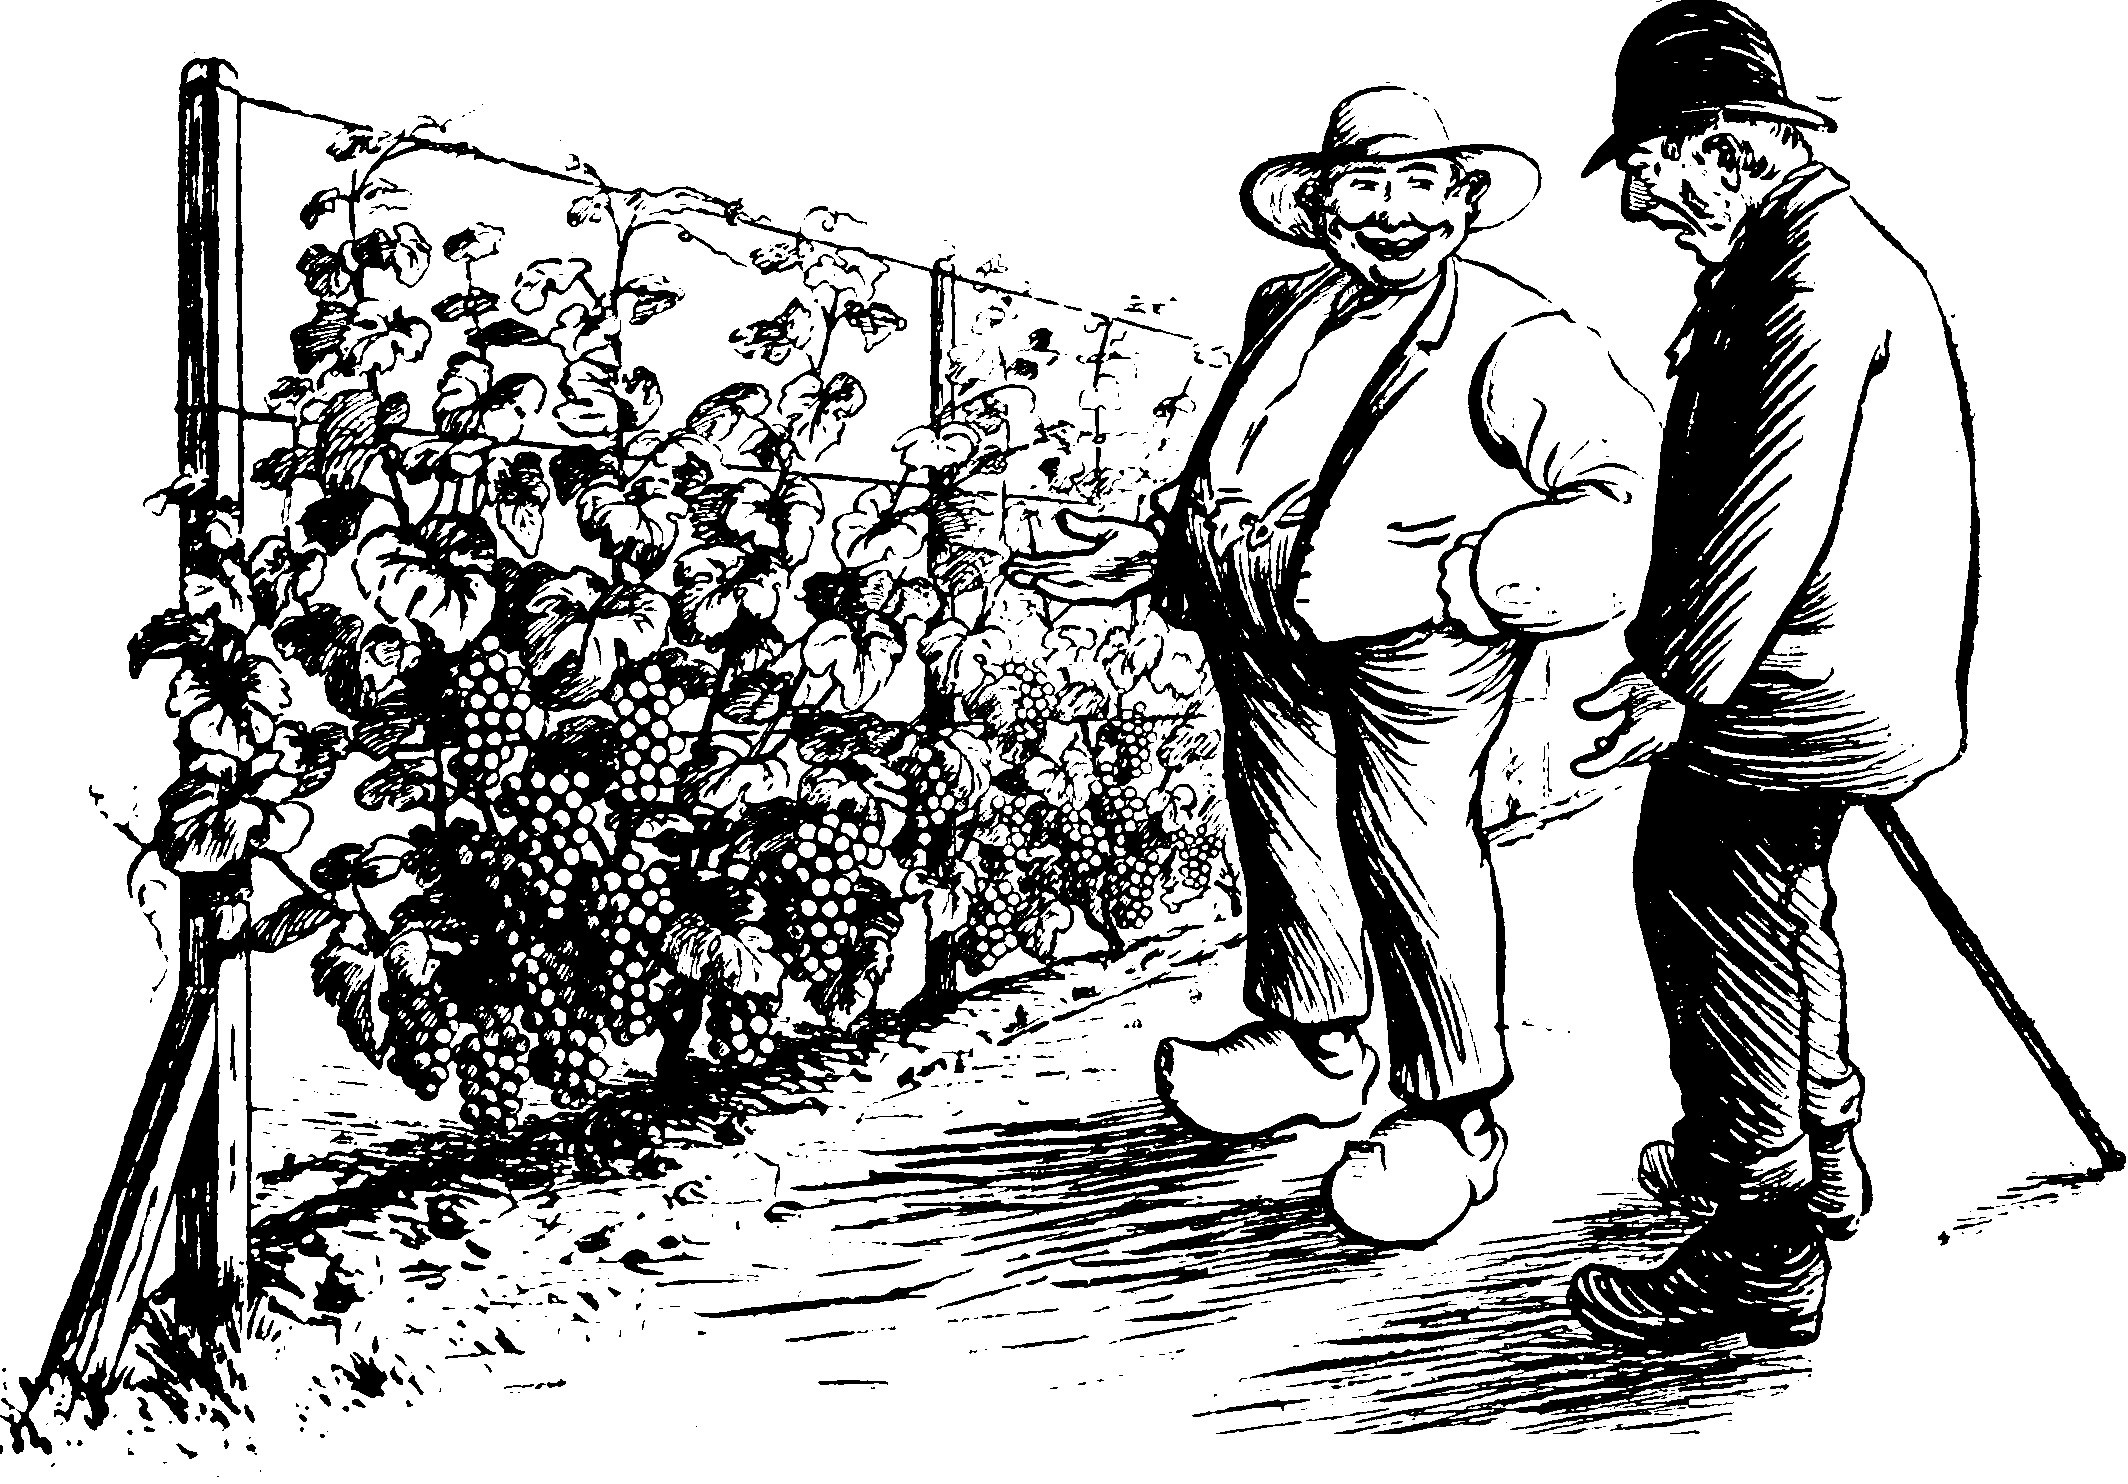
\includegraphics[width=0.7\textwidth]{images/brev5.png}
\end{center}
\breakpage